\subsection{Interrelación Centro - Titulación}

   \begin{description}
      \item[Definición] En esta interrelación se deja constancia de que cada
      centro establecido en el sistema podrá disponer de varias titulaciones.

      \item[Características] La interrelación presenta las siguientes
                             características:

         \begin{itemize}
            \item \textbf{Nombre:} C-T
            \item \textbf{Tipo de la interrelación:} El tipo de entidad
                  Titulación es débil por identificación respecto al tipo de
                  entidad Centro.
            \item \textbf{Cardinalidad de la interrelación:} 1:N
                  \begin{itemize}
                     \item Centro: dispone\_de (0,n)
                     \item Titulación: pertenece\_a (1,1)
                  \end{itemize}
            \item \textbf{Número de atributos:} Ninguno.
         \end{itemize}

      \item[Diagrama] La figura \ref{diagramaC-T} muestra el diagrama de la
                      interrelación.
      \item \begin{figure}[!ht]
            \begin{center}
            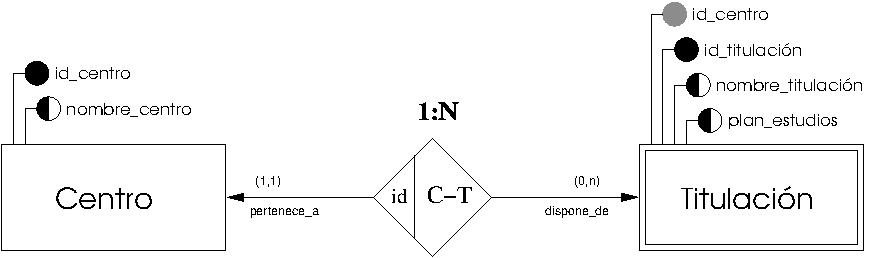
\includegraphics[]{07.Modelo_Entidad-Interrelacion/7.3.Analisis_Interrelaciones/diagramas/C-T.pdf}
            \caption{Diagrama de la interrelación C-T.}
            \label{diagramaC-T}
            \end{center}
         \end{figure}

      \item[Ejemplo práctico del tipo de interrelación]

      \item \begin{center}
            \begin{tabular}{ | c | c | }
            \hline
            \multicolumn{2}{ | c | }{\textbf{Tipo de interrelación C-T}} \\
            \hline
            \textbf{Centro} & \textbf{Titulación}\\
            \hline
            id\_centro & id\_centro+id\_titulación \\
            \hline
            15 & 153 \\
            \hline
            \end{tabular}
         \end{center}

   \end{description}
